\heading{数据结构与算法B-模拟题1-期末}
\textbf{一、选择题（每小题 3 分，共 30 分）}

\begin{question}
数据结构的三个基本要素是（\quad）。
\begin{choiceoptions}[2]
  \item 顺序结构、链式结构、散列结构
  \item 逻辑结构、存储结构、算法
  \item 线性结构、树型结构、图状结构
  \item 以上都不是
\end{choiceoptions}
\begin{solution}
选 B。数据结构三要素为逻辑结构、存储结构和算法（数据操作）。
\end{solution}
\end{question}

\begin{question}
栈是一种后进先出表。若入栈的顺序为 $\{1,2,3,4\}$，则出栈的顺序不可能是（\quad）。
\begin{choiceoptions}[2]
  \item $1234$
  \item $1243$
  \item $1423$
  \item $2134$
\end{choiceoptions}
\begin{solution}
选 C。$1423$ 不可能：要 $4$ 在 $2$ 之前出栈，则 $4$ 入栈时 $2,3$ 已在栈中，出栈顺序应为 $4,3,2$ 而非 $4,2,3$。
\end{solution}
\end{question}

\begin{question}
用一个大小为 $6$ 的数组来实现环形队列，元素从下标 $0$ 开始存放。当前 front 和 rear 的值分别为 $4$ 和 $1$，现在从队列中删除一个元素，再增加两个元素，则 front 和 rear 的值为（\quad）。
\begin{choiceoptions}[1]
  \item $0,\;2$
  \item $5,\;3$
  \item $0,\;1$
  \item $5,\;2$
\end{choiceoptions}
\begin{solution}
选 B。环形队列删除：front = (4+1)\%6 = 5。增加两个：rear = (1+2)\%6 = 3。
\end{solution}
\end{question}

\begin{question}
假定一棵二叉树的结点个数为 $33$ 个，定义根结点的层数为 $0$，则它的高度最小为（\quad）。
\begin{choiceoptions}[2]
  \item $5$
  \item $6$
  \item $7$
  \item $4$
\end{choiceoptions}
\begin{solution}
选 A。根结点层数为 $0$ 时，含 $33$ 个结点的二叉树最小最大层数为 $5$，因为前 $5$ 层最多有 $2^5-1=31$ 个结点，而前 $6$ 层最多有 $2^6-1=63$ 个结点。
\end{solution}
\end{question}

\begin{question}
已知某二叉树的先根周游序列为 $\{A,B,D,E,C\}$，中根周游序列为 $\{D,B,E,A,C\}$，则该二叉树的后根周游序列是（\quad）。
\begin{choiceoptions}[2]
  \item $\{A,B,C,D,E\}$
  \item $\{D,B,E,C,A\}$
  \item $\{C,D,E,B,A\}$
  \item $\{D,E,B,C,A\}$
\end{choiceoptions}
\begin{solution}
选 D。由先序确定根 $A$，中序划分左子树 $\{D,B,E\}$、右子树 $\{C\}$。递归可得后序：$D,E,B,C,A$。
\end{solution}
\end{question}

\begin{question}
在待排序的元素序列基本有序的前提下，下列空间效率最差的排序方法是（\quad）。
\begin{choiceoptions}[2]
  \item 直接插入排序
  \item 选择排序
  \item 快速排序
  \item 冒泡排序
\end{choiceoptions}
\begin{solution}
选 C。快速排序在基本有序时递归深度 $O(n)$，空间复杂度 $O(n)$，远高于其他 $O(1)$。
\end{solution}
\end{question}

\begin{question}
在平均情况下，下列时间复杂度最好的排序方法是（\quad）。
\begin{choiceoptions}[2]
  \item 直接插入排序（平均 $O(n^2)$）
  \item 选择排序（平均 $O(n^2)$）
  \item 快速排序（平均 $O(n\log n)$）
  \item 冒泡排序（平均 $O(n^2)$）
\end{choiceoptions}
\begin{solution}
选 C。快速排序平均时间复杂度 $O(n\log n)$。
\end{solution}
\end{question}

\begin{question}
下列关于图的说法不正确的是（\quad）。
\begin{choiceoptions}[2]
  \item 用邻接矩阵法存储一个图时，其存储空间与图的边数无关
  \item AOV 网络拓扑排序的结果是唯一的
  \item 强连通分量是有向图中的极大强连通子图
  \item 一个有向图的邻接表和逆邻接表中的结点个数一定相等
\end{choiceoptions}
\begin{solution}
选 B。拓扑排序结果不一定唯一，取决于入度为 $0$ 的顶点选择顺序。
\end{solution}
\end{question}

\begin{question}
AVL 树是一种（\quad）。
\begin{choiceoptions}[2]
  \item 生成树
  \item 平衡树
  \item B 树
  \item 二叉排序树
\end{choiceoptions}
\begin{solution}
选 B。AVL 树是平衡二叉搜索树（任一结点左右子树高度差 $\le1$）。
\end{solution}
\end{question}

\begin{question}
任何一个无向连通图的最小生成树（\quad）。
\begin{choiceoptions}[2]
  \item 只有一棵
  \item 有一棵或多棵
  \item 一定有多棵
  \item 可能不存在
\end{choiceoptions}
\begin{solution}
选 B。当图中有权值相等的边时，最小生成树可能不唯一。
\end{solution}
\end{question}

\clearpage

\textbf{二、解答题（共 40 分）}

\begin{question}[线性表存储结构比较]（8 分）

请说明线性表的顺序存储（顺序表）与链式存储（单链表）的异同，比较它们的优缺点。当字典采用二分法进行检索时，应采用哪一种存储结构？

\begin{solution}
\begin{itemize}
  \item 顺序表：逻辑上相邻的元素在物理上也相邻，支持随机访问 $O(1)$，插入/删除需移动元素 $O(n)$。
  \item 单链表：逻辑上相邻的元素物理上不一定相邻，通过引用链接，不支持随机访问 $O(n)$，插入/删除只需修改引用 $O(1)$。
  \item 二分法检索需要随机访问中间元素，应采用顺序表。
\end{itemize}
\end{solution}
\end{question}

\begin{question}[Huffman编码]（10 分）

字符串 \texttt{"this sentence is used for test"}，请使用 Huffman 编码方式对该字符串中的所有字符重新编码，以实现对它的压缩，给出编码过程中实现的 Huffman 树以及字符 \texttt{'s'} 的编码结果。

\begin{solution}
先统计字符频率：空格、\texttt{e}、\texttt{s} 各 $5$ 次，\texttt{t} 为 $4$ 次，\texttt{i}、\texttt{n} 各 $2$ 次，\texttt{c,d,f,h,o,r,u} 各 $1$ 次。Huffman 编码不唯一，下面给出一种合法编码：
\begin{center}
\resizebox{0.98\linewidth}{!}{%
\begin{tikzpicture}[
  level distance=11mm,
  level 1/.style={sibling distance=88mm},
  level 2/.style={sibling distance=50mm},
  level 3/.style={sibling distance=31mm},
  level 4/.style={sibling distance=21mm},
  level 5/.style={sibling distance=15mm},
  every node/.style={draw,rounded corners=1pt,align=center,font=\scriptsize,inner sep=1.3pt}
]
\node {30}
  child {node {12}
    child {node {\texttt{s}:5}}
    child {node {7}
      child {node {3}
        child {node {\texttt{u}:1}}
        child {node {\texttt{i}:2}}
      }
      child {node {\texttt{t}:4}}
    }
  }
  child {node {18}
    child {node {8}
      child {node {4}
        child {node {\texttt{n}:2}}
        child {node {2}
          child {node {\texttt{c}:1}}
          child {node {\texttt{d}:1}}
        }
      }
      child {node {4}
        child {node {2}
          child {node {\texttt{f}:1}}
          child {node {\texttt{h}:1}}
        }
        child {node {2}
          child {node {\texttt{o}:1}}
          child {node {\texttt{r}:1}}
        }
      }
    }
    child {node {10}
      child {node {空格:5}}
      child {node {\texttt{e}:5}}
    }
  };
\end{tikzpicture}
}%
\end{center}
\begin{center}
\begin{tabular}{c|ccccccccccccc}
\toprule
字符 & 空格 & c & d & e & f & h & i & n & o & r & s & t & u \\
\midrule
频率 & 5 & 1 & 1 & 5 & 1 & 1 & 2 & 2 & 1 & 1 & 5 & 4 & 1 \\
编码 & 110 & 10010 & 10011 & 111 & 10100 & 10101 & 0101 & 1000 & 10110 & 10111 & 00 & 011 & 0100 \\
\bottomrule
\end{tabular}
\end{center}
因此在这棵 Huffman 树中，字符 \texttt{s} 的编码可取 \texttt{00}。若合并等权结点的先后不同，具体码字会变，但频率高的字符码长较短这一结论不变。
\end{solution}
\end{question}

\begin{question}[排序算法]（12 分）

对待排序的关键码集合 $\{E,C,A,M,S,R,D,F\}$ 按升序排序，请叙述直接插入排序、堆排序、快速排序、归并排序的基本思路，以及它们对上述数组第一趟扫描后的结果（快速排序使用第一个元素作为分界点）。

\begin{solution}
四种算法的第一趟结果如下表。这里“快速排序第一趟”按第一个元素 $E$ 为枢轴、左右交替扫描的常见划分过程给出；“堆排序第一趟”常有两种口径，表中同时列出。
\begin{center}
\begin{tabular}{@{}p{0.24\linewidth} p{0.66\linewidth}@{}}
\toprule
算法 & 第一趟后的序列 \\
\midrule
直接插入排序 & $C,E,A,M,S,R,D,F$ \\
堆排序（建成大根堆） & $S,M,R,F,C,A,D,E$ \\
堆排序（建堆后再输出一次最大值） & $R,M,E,F,C,A,D,S$ \\
快速排序 & $D,C,A,E,S,R,M,F$ \\
归并排序 & $C,E,A,M,R,S,D,F$ \\
\bottomrule
\end{tabular}
\end{center}
\end{solution}
\end{question}

\begin{question}[最短路径]（10 分）

下面是一个带权有向图的邻接矩阵表示（$\infty$ 表示无边），试画出该图结构，并给出该图中由 $V_0$ 到 $V_4$ 的最短路径。
\[
\begin{pmatrix}
0&50&10&\infty&45&\infty\\
\infty&0&15&\infty&5&\infty\\
20&\infty&0&15&\infty&\infty\\
\infty&20&\infty&0&35&\infty\\
\infty&\infty&\infty&30&0&\infty\\
\infty&\infty&\infty&3&\infty&0
\end{pmatrix}
\]
\begin{center}
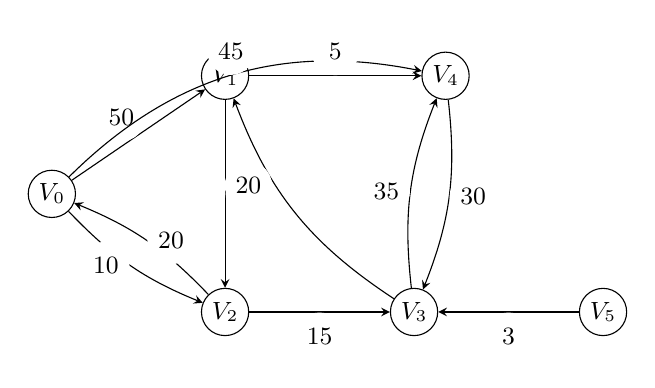
\begin{tikzpicture}[x=10mm,y=10mm,every node/.style={draw,circle,font=\small,minimum size=6mm,inner sep=0pt},>=stealth]
\node (v0) at (0,1) {$V_0$};
\node (v1) at (2.2,2.5) {$V_1$};
\node (v2) at (2.2,-0.5) {$V_2$};
\node (v3) at (4.6,-0.5) {$V_3$};
\node (v4) at (5,2.5) {$V_4$};
\node (v5) at (7,-0.5) {$V_5$};
\draw[->] (v0)--node[above left,draw=none,fill=white]{50}(v1);
\draw[->] (v0) to[bend right=12] node[left,draw=none,fill=white]{10}(v2);
\draw[->] (v0) to[bend left=28] node[above,draw=none,fill=white]{45}(v4);
\draw[->] (v1)--node[right,draw=none,fill=white]{15}(v2);
\draw[->] (v1)--node[above,draw=none,fill=white]{5}(v4);
\draw[->] (v2) to[bend right=12] node[right,draw=none,fill=white]{20}(v0);
\draw[->] (v2)--node[below,draw=none,fill=white]{15}(v3);
\draw[->] (v3) to[bend left=18] node[pos=0.72,below left,draw=none,fill=white]{20}(v1);
\draw[->] (v3) to[bend left=14] node[left,draw=none,fill=white]{35}(v4);
\draw[->] (v4) to[bend left=14] node[right,draw=none,fill=white]{30}(v3);
\draw[->] (v5)--node[below,draw=none,fill=white]{3}(v3);
\end{tikzpicture}
\end{center}

\begin{solution}
由矩阵可得有向边：$V_0\to V_1(50)$、$V_0\to V_2(10)$、$V_0\to V_4(45)$、$V_1\to V_2(15)$、$V_1\to V_4(5)$、$V_2\to V_0(20)$、$V_2\to V_3(15)$、$V_3\to V_1(20)$、$V_3\to V_4(35)$、$V_4\to V_3(30)$、$V_5\to V_3(3)$。从 $V_0$ 执行 Dijkstra 算法：
\begin{center}
\small
\begin{tabular}{c c c c}
\toprule
步骤 & 确定顶点 & 当前距离 $(d_1,d_2,d_3,d_4,d_5)$ & 前驱更新 \\
\midrule
初始 & $V_0$ & $(50,10,\infty,45,\infty)$ & $pre_1=0,pre_2=0,pre_4=0$ \\
1 & $V_2$ & $(50,10,25,45,\infty)$ & $pre_3=2$ \\
2 & $V_3$ & $(45,10,25,45,\infty)$ & $pre_1=3$ \\
3 & $V_1$ & $(45,10,25,45,\infty)$ & 无更新 \\
4 & $V_4$ & $(45,10,25,45,\infty)$ & 完成 \\
\bottomrule
\end{tabular}
\end{center}
故最短路径为 $V_0\to V_4$，长度为 $45$。顶点 $V_5$ 从 $V_0$ 不可达，不影响该最短路径。
\end{solution}
\end{question}

\clearpage

\textbf{三、算法填空（共 10 分）}



\begin{question}[散列表检索]（10 分）

完成下列 Python 散列表检索算法。设散列函数为 \texttt{h}，采用线性探查法解决冲突；\texttt{EMPTY} 表示空位置。函数返回二元组 \texttt{(found, position)}，其中 \texttt{found} 表示是否检索成功，\texttt{position} 表示查找成功位置或首次空位位置。

\begin{pycode}
EMPTY = None


def linear_search(table, key, h):
    m = len(table)
    d = __________                              # (1) 初始散列地址
    for _ in range(m):
        entry = table[d]
        if entry is not EMPTY and __________:   # (2) 检索成功
            __________                          # (3) 记录位置
            return True, position
        if entry is EMPTY:
            return False, d
        __________                              # (4) 线性探查下一地址
    __________                                  # (5) 散列表已探查一周
\end{pycode}

\begin{solution}
填空答案：
\begin{enumerate}
  \item \texttt{h(key) \% m}
  \item \texttt{entry.key == key}
  \item \texttt{position = d}
  \item \texttt{d = (d + 1) \% m}
  \item \texttt{return False, None}
\end{enumerate}
线性探查从散列地址 \texttt{h(key) \% m} 开始；若当前位置非空且关键字等于待查关键字，则查找成功。若遇到空位置，说明关键字不在表中且可插入该位置；否则地址加 $1$ 后对表长取模继续探查。若探查一周仍未找到且未遇到空位，则散列表已满，返回查找失败。
\end{solution}
\end{question}
\clearpage

\textbf{四、算法设计（共 20 分）}



\begin{question}[求子树深度]（20 分）

已知一棵树采用孩子兄弟表示法。请用 Python 设计函数，求树中以值为 $x$ 的结点为根的子树深度。限定：值为 $x$ 的结点在树中最多有一个。注意栈或队列等辅助结构可以直接引用，不用自己定义。

\begin{pycode}
class CSNode:
    def __init__(self, info):
        self.info = info          # 结点数据
        self.first_child = None   # 第一个孩子
        self.next_sibling = None  # 下一个兄弟

p_mytree = ...                    # 树根引用
\end{pycode}

\begin{solution}
采用深度优先搜索：先在整棵树中寻找值为 $x$ 的结点；若找到，再从该结点出发计算子树深度。孩子兄弟表示中，\texttt{first\_child} 引用第一个孩子，\texttt{next\_sibling} 引用下一个兄弟。

参考实现如下（结点不存在时返回 $0$）：
\begin{quote}
\footnotesize
\begin{tabular}{@{}l@{}}
\texttt{def subtree\_height(root):}\\
\texttt{\quad if root is None:}\\
\texttt{\quad\quad return 0}\\
\texttt{\quad best = 0}\\
\texttt{\quad child = root.first\_child}\\
\texttt{\quad while child is not None:}\\
\texttt{\quad\quad best = max(best, subtree\_height(child))}\\
\texttt{\quad\quad child = child.next\_sibling}\\
\texttt{\quad return best + 1}\\[0.35em]
\texttt{def find\_node(root, x):}\\
\texttt{\quad if root is None:}\\
\texttt{\quad\quad return None}\\
\texttt{\quad if root.info == x:}\\
\texttt{\quad\quad return root}\\
\texttt{\quad child = root.first\_child}\\
\texttt{\quad while child is not None:}\\
\texttt{\quad\quad ans = find\_node(child, x)}\\
\texttt{\quad\quad if ans is not None:}\\
\texttt{\quad\quad\quad return ans}\\
\texttt{\quad\quad child = child.next\_sibling}\\
\texttt{\quad return None}\\[0.35em]
\texttt{target = find\_node(p\_mytree, x)}\\
\texttt{answer = 0 if target is None else subtree\_height(target)}
\end{tabular}
\end{quote}
\texttt{find\_node} 会沿“第一个孩子--下一个兄弟”结构搜索整棵树；\texttt{subtree\_height} 枚举当前结点的所有孩子，取孩子子树高度最大值后加 $1$，因此得到的就是目标子树深度。
\end{solution}
\end{question}

\clearpage
